\section{Problem (4)}
	In the \cref{fig:hwb_problem4}, three particles of mass $m = 3.2 \ kg$ are fastened to three rods of length $d = 0.45 \ m$ and negligible mass. The rigid assembly rotates about point $O$ at angular speeed $\omega = \ 9.0 \ rad/s$. About $O$,

	\begin{figure}[H]
		\begin{center}
			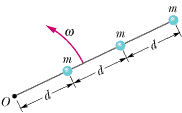
\includegraphics[scale=1]{hwb_problem4}
			\caption{Illustration of Problem 4}
			\label{fig:hwb_problem4}
		\end{center}
	\end{figure}

	\subsection{Question (a)}

		What is the rotational inertia of the assembly?

		\textbf{R:}

		\begin{align}
			x
		\end{align}

	\subsection{Question (b)}

		What is the magnitude of the angular momentum of the asembly?

		\textbf{R:}

		\begin{align}
			x
		\end{align}
